\documentclass[aspectratio=169, 11pt]{beamer}

\usetheme{Madrid}
\usecolortheme{seahorse}
\setbeamertemplate{navigation symbols}{}
\setbeamertemplate{footline}[frame number]
\setbeamertemplate{itemize items}[circle]

\usepackage{amsmath}
\usepackage{amssymb}
\usepackage{xcolor}
\usepackage{tikz}
\usetikzlibrary{arrows.meta, positioning, calc, decorations.pathreplacing, shapes.geometric, fit}
\usepackage{booktabs}
\usepackage{graphicx}

% Custom colors
\definecolor{cblue}{RGB}{66,133,244}
\definecolor{cred}{RGB}{234,67,53}
\definecolor{cgreen}{RGB}{52,168,83}
\definecolor{cyellow}{RGB}{251,188,4}
\definecolor{cpurple}{RGB}{153,51,255}
\definecolor{lightblue}{RGB}{220,235,252}
\definecolor{lightred}{RGB}{252,225,222}
\definecolor{lightgreen}{RGB}{222,247,226}
\definecolor{lightpurple}{RGB}{237,222,252}
\definecolor{lightyellow}{RGB}{255,248,220}
\definecolor{darkbg}{RGB}{40,44,52}

\title{\textbf{Classifier-Free Guidance (CFG)}}
\subtitle{A Visual Introduction for Beginners}
\author{Pan Changxun \quad 2024011323}
\date{Spring 2026}

\begin{document}

% ============================================================
% Title
% ============================================================
\begin{frame}
\titlepage
\end{frame}

% ============================================================
\begin{frame}{Outline}
\tableofcontents
\end{frame}

% ============================================================
\section{Motivation: Why Do We Need Guidance?}
% ============================================================

\begin{frame}{The Problem: Conditional Generation}

\begin{columns}
\begin{column}{0.55\textwidth}
We want a diffusion model to generate images \textbf{matching a text prompt}.

\bigskip
\textbf{Example:}
\begin{itemize}
    \item Prompt: ``a photo of a cat''
    \item Model should generate: a realistic cat image
    \item Model should \textbf{NOT} generate: random noise, a dog, or a blurry mess
\end{itemize}

\bigskip
\alert{Challenge:} Naive conditional models often produce outputs that are \emph{correct but bland} --- they lack fidelity and sharpness.
\end{column}

\begin{column}{0.4\textwidth}
\centering
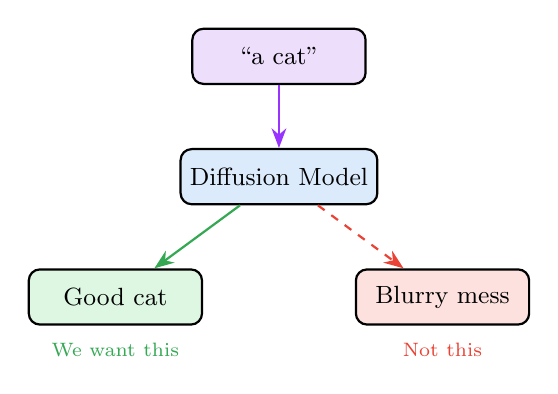
\begin{tikzpicture}[
    >={Stealth[length=2.5mm]},
    box/.style={draw, rounded corners, minimum width=2.2cm, minimum height=0.7cm, font=\small, thick},
]
    \node[box, fill=lightpurple] (prompt) {``a cat''};
    \node[box, fill=lightblue, below=0.8cm of prompt] (model) {Diffusion Model};
    \node[box, fill=lightgreen, below left=0.8cm and -0.3cm of model] (good) {Good cat};
    \node[box, fill=lightred, below right=0.8cm and -0.3cm of model] (bad) {Blurry mess};

    \draw[->, thick, cpurple] (prompt) -- (model);
    \draw[->, thick, cgreen] (model) -- (good);
    \draw[->, thick, cred, dashed] (model) -- (bad);

    \node[cgreen, font=\scriptsize, below=0.1cm of good] {We want this};
    \node[cred, font=\scriptsize, below=0.1cm of bad] {Not this};
\end{tikzpicture}
\end{column}
\end{columns}

\end{frame}

% ============================================================
\begin{frame}{Two Approaches to Guidance}

\begin{center}
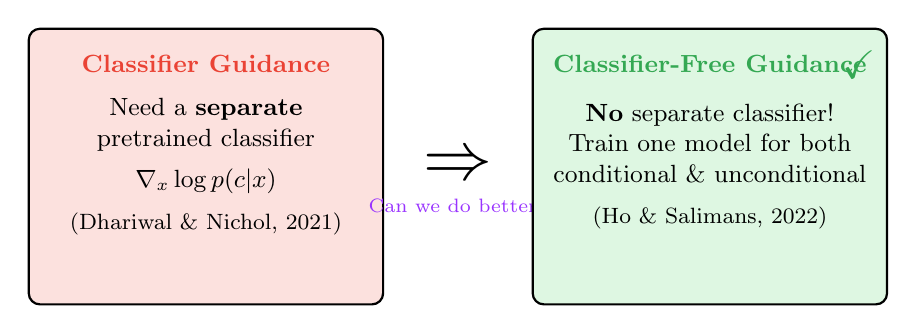
\begin{tikzpicture}[
    >={Stealth[length=2.5mm]},
    bigbox/.style={draw, rounded corners, thick, minimum width=4.5cm, minimum height=3.5cm, align=center},
    label/.style={font=\small\bfseries},
]
    % Classifier Guidance
    \node[bigbox, fill=lightred] (cg) at (0,0) {};
    \node[label, cred] at (0, 1.3) {Classifier Guidance};
    \node[align=center, font=\small] at (0, 0) {
        Need a \textbf{separate}\\
        pretrained classifier\\[4pt]
        $\nabla_x \log p(c|x)$\\[4pt]
        {\footnotesize (Dhariwal \& Nichol, 2021)}
    };

    % Arrow
    \node[font=\Huge] at (3.2, 0) {$\Rightarrow$};
    \node[font=\scriptsize, cpurple] at (3.2, -0.5) {Can we do better?};

    % Classifier-Free Guidance
    \node[bigbox, fill=lightgreen] (cfg) at (6.4,0) {};
    \node[label, cgreen] at (6.4, 1.3) {Classifier-Free Guidance};
    \node[align=center, font=\small] at (6.4, 0) {
        \textbf{No} separate classifier!\\
        Train one model for both\\
        conditional \& unconditional\\[4pt]
        {\footnotesize (Ho \& Salimans, 2022)}
    };

    % Checkmark
    \node[cgreen, font=\Large] at (8.3, 1.3) {\checkmark};
\end{tikzpicture}
\end{center}

\bigskip
\centering
\textbf{Classifier-Free Guidance (CFG)} achieves strong guidance\\
\emph{without} needing any external classifier.
\end{frame}

% ============================================================
\section{Background: Diffusion Models Refresher}
% ============================================================

\begin{frame}{Diffusion Models in 30 Seconds}

\begin{center}
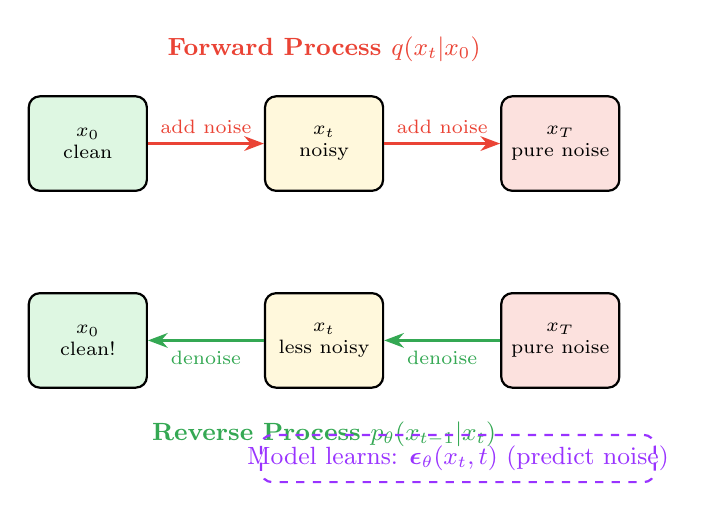
\begin{tikzpicture}[
    >={Stealth[length=2.5mm]},
    imgbox/.style={draw, rounded corners, minimum width=1.5cm, minimum height=1.2cm, thick, font=\scriptsize, align=center},
]
    % Forward process
    \node[imgbox, fill=lightgreen] (x0) at (0, 1.5) {$x_0$\\clean};
    \node[imgbox, fill=lightyellow] (x1) at (3, 1.5) {$x_t$\\noisy};
    \node[imgbox, fill=lightred] (xT) at (6, 1.5) {$x_T$\\pure noise};

    \draw[->, thick, cred] (x0) -- node[above, font=\scriptsize] {add noise} (x1);
    \draw[->, thick, cred] (x1) -- node[above, font=\scriptsize] {add noise} (xT);

    \node[cred, font=\small\bfseries, above=0.3cm of x1] {Forward Process $q(x_t|x_0)$};

    % Reverse process
    \node[imgbox, fill=lightred] (xT2) at (6, -1) {$x_T$\\pure noise};
    \node[imgbox, fill=lightyellow] (x12) at (3, -1) {$x_t$\\less noisy};
    \node[imgbox, fill=lightgreen] (x02) at (0, -1) {$x_0$\\clean!};

    \draw[->, thick, cgreen] (xT2) -- node[below, font=\scriptsize] {denoise} (x12);
    \draw[->, thick, cgreen] (x12) -- node[below, font=\scriptsize] {denoise} (x02);

    \node[cgreen, font=\small\bfseries, below=0.3cm of x12] {Reverse Process $p_\theta(x_{t-1}|x_t)$};

    % The model
    \draw[thick, dashed, cpurple, rounded corners] (2.2, -2.2) rectangle (7.2, -2.8);
    \node[font=\small, cpurple] at (4.7, -2.5) {Model learns: $\boldsymbol{\epsilon}_\theta(x_t, t)$ (predict noise)};
\end{tikzpicture}
\end{center}

\bigskip

\textbf{Key idea:} The model $\boldsymbol{\epsilon}_\theta(x_t, t)$ predicts the noise $\epsilon$ that was added to get $x_t$, then we subtract it to denoise step-by-step.

\end{frame}

% ============================================================
\begin{frame}{Conditional Diffusion Models}

To generate images conditioned on a label/text $c$, we train:
\[
    \boldsymbol{\epsilon}_\theta(x_t, t, c) \quad \longleftarrow \quad \text{``predict noise, given noisy image } x_t \text{, timestep } t \text{, and condition } c\text{''}
\]

\begin{center}
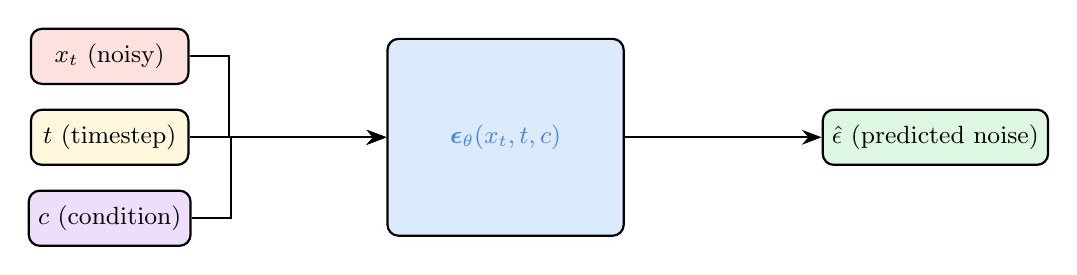
\begin{tikzpicture}[
    >={Stealth[length=2.5mm]},
    box/.style={draw, rounded corners, minimum width=2cm, minimum height=0.7cm, font=\small, thick},
]
    \node[box, fill=lightred] (xt) {$x_t$ (noisy)};
    \node[box, fill=lightyellow, below=0.3cm of xt] (t) {$t$ (timestep)};
    \node[box, fill=lightpurple, below=0.3cm of t] (c) {$c$ (condition)};

    \node[box, fill=lightblue, right=2.5cm of t, minimum width=3cm, minimum height=2.5cm] (model) {};
    \node[font=\small\bfseries, cblue] at (model) {$\boldsymbol{\epsilon}_\theta(x_t, t, c)$};

    \node[box, fill=lightgreen, right=2.5cm of model] (out) {$\hat{\epsilon}$ (predicted noise)};

    \draw[->, thick] (xt.east) -- ++(0.5,0) |- (model.west);
    \draw[->, thick] (t) -- (model);
    \draw[->, thick] (c.east) -- ++(0.5,0) |- (model.west);
    \draw[->, thick] (model) -- (out);
\end{tikzpicture}
\end{center}

\bigskip
\alert{Problem:} This alone often doesn't produce images that strongly match the condition $c$. We need a way to \textbf{amplify} the effect of the condition.

\end{frame}

% ============================================================
\section{Classifier Guidance (The Predecessor)}
% ============================================================

\begin{frame}{Classifier Guidance: The Idea}

\textbf{Dhariwal \& Nichol (2021)} proposed using a pretrained classifier $p_\phi(c|x_t)$ to guide the diffusion process.

\bigskip

The score function of a conditional model can be decomposed via Bayes' rule:
\begin{align}
    \nabla_{x_t} \log p(x_t | c)
    &= \nabla_{x_t} \log p(x_t) + \nabla_{x_t} \log p(c | x_t) \nonumber
\end{align}

\begin{center}
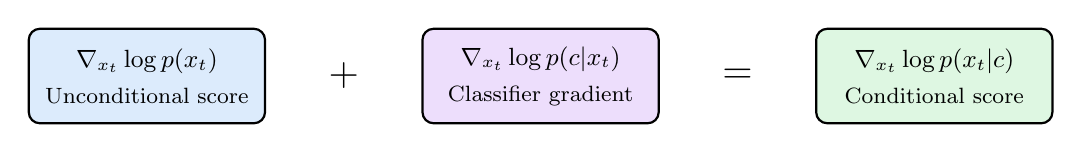
\begin{tikzpicture}[
    >={Stealth[length=2.5mm]},
    termbox/.style={draw, rounded corners, thick, minimum width=3cm, minimum height=1.2cm, align=center, font=\small},
]
    \node[termbox, fill=lightblue] (uncond) at (0,0) {
        $\nabla_{x_t} \log p(x_t)$\\[2pt]
        \footnotesize Unconditional score
    };
    \node[font=\Large] at (2.5,0) {$+$};
    \node[termbox, fill=lightpurple] (cls) at (5,0) {
        $\nabla_{x_t} \log p(c|x_t)$\\[2pt]
        \footnotesize Classifier gradient
    };
    \node[font=\Large] at (7.5,0) {$=$};
    \node[termbox, fill=lightgreen] (cond) at (10,0) {
        $\nabla_{x_t} \log p(x_t|c)$\\[2pt]
        \footnotesize Conditional score
    };
\end{tikzpicture}
\end{center}

\bigskip
Add a guidance scale $s$ to strengthen the classifier signal:
\[
    \tilde{\nabla}_{x_t} = \nabla_{x_t} \log p(x_t) + \alert{s} \cdot \nabla_{x_t} \log p(c|x_t)
\]

\end{frame}

% ============================================================
\begin{frame}{Classifier Guidance: The Drawbacks}

\begin{columns}
\begin{column}{0.5\textwidth}
\textbf{Downsides:}
\begin{enumerate}
    \item Need to train a \textbf{separate classifier} on noisy images $x_t$ at every noise level
    \item The classifier must handle \textbf{all noise levels} $t = 1, \ldots, T$
    \item Classifier gradients can be \textbf{adversarial} --- pushing images toward classifier-fooling artifacts
    \item More complex pipeline: two models to maintain
\end{enumerate}
\end{column}

\begin{column}{0.45\textwidth}
\centering
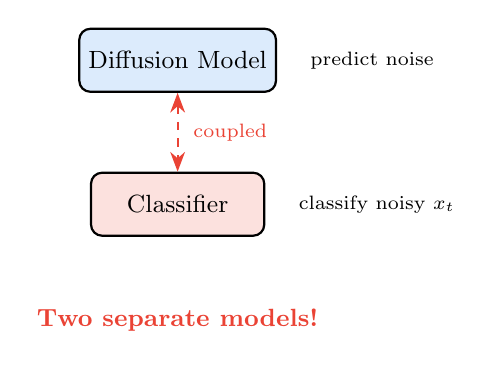
\begin{tikzpicture}[
    >={Stealth[length=2.5mm]},
    box/.style={draw, rounded corners, minimum width=2.2cm, minimum height=0.8cm, font=\small, thick},
]
    \node[box, fill=lightblue] (diff) {Diffusion Model};
    \node[box, fill=lightred, below=1cm of diff] (cls) {Classifier};

    \node[font=\scriptsize, right=0.3cm of diff] {predict noise};
    \node[font=\scriptsize, right=0.3cm of cls] {classify noisy $x_t$};

    \draw[<->, thick, dashed, cred] (diff) -- node[right, font=\scriptsize, xshift=2pt] {coupled} (cls);

    \node[cred, font=\small\bfseries, below=0.8cm of cls] {Two separate models!};
\end{tikzpicture}

\bigskip
\alert{Can we get the same guidance effect with just \emph{one} model?}
\end{column}
\end{columns}

\end{frame}

% ============================================================
\section{Classifier-Free Guidance: The Core Idea}
% ============================================================

\begin{frame}{The Key Insight}

\begin{block}{Core Observation}
From Bayes' rule: $\;\nabla_{x_t} \log p(c|x_t) = \nabla_{x_t} \log p(x_t|c) - \nabla_{x_t} \log p(x_t)$
\end{block}

\bigskip
Substitute back into the guided score:
\begin{align}
    \tilde{\nabla}_{x_t}
    &= \nabla_{x_t}\log p(x_t) + s\cdot\Big[\nabla_{x_t}\log p(x_t|c) - \nabla_{x_t}\log p(x_t)\Big] \nonumber \\[6pt]
    &= \underbrace{(1-s)\cdot\nabla_{x_t}\log p(x_t)}_{\text{unconditional}} + \underbrace{s\cdot\nabla_{x_t}\log p(x_t|c)}_{\text{conditional}} \nonumber
\end{align}

\bigskip
\begin{alertblock}{No Classifier Needed!}
We only need:
\begin{enumerate}
    \item An \textbf{unconditional} score $\nabla_{x_t}\log p(x_t)$ \quad $\Leftrightarrow$ \quad $\boldsymbol{\epsilon}_\theta(x_t, t)$
    \item A \textbf{conditional} score $\nabla_{x_t}\log p(x_t|c)$ \quad $\Leftrightarrow$ \quad $\boldsymbol{\epsilon}_\theta(x_t, t, c)$
\end{enumerate}
Both can come from the \textbf{same} diffusion model!
\end{alertblock}

\end{frame}

% ============================================================
\begin{frame}{The CFG Formula}

In terms of the noise prediction network $\boldsymbol{\epsilon}_\theta$:

\[
\boxed{
    \tilde{\boldsymbol{\epsilon}}_\theta(x_t, t, c)
    = \underbrace{\boldsymbol{\epsilon}_\theta(x_t, t, \varnothing)}_{\text{unconditional}}
    + w \cdot \Big(\underbrace{\boldsymbol{\epsilon}_\theta(x_t, t, c)}_{\text{conditional}} - \underbrace{\boldsymbol{\epsilon}_\theta(x_t, t, \varnothing)}_{\text{unconditional}}\Big)
}
\]

where $w \geq 0$ is the \textbf{guidance scale} and $\varnothing$ denotes ``no condition'' (null/empty).

\bigskip

\begin{center}
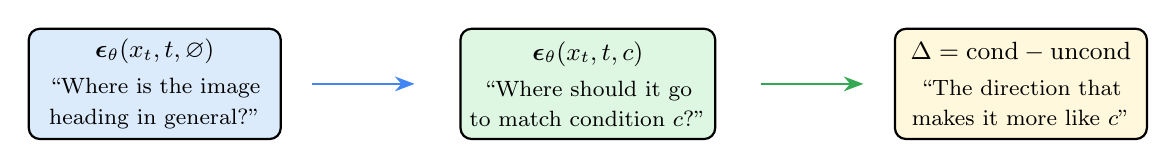
\begin{tikzpicture}[
    >={Stealth[length=2.5mm]},
    termbox/.style={draw, rounded corners, thick, minimum width=3.2cm, minimum height=1.4cm, align=center, font=\small},
]
    \node[termbox, fill=lightblue] (uncond) at (0,0) {
        $\boldsymbol{\epsilon}_\theta(x_t, t, \varnothing)$\\[2pt]
        \footnotesize ``Where is the image\\
        \footnotesize heading in general?''
    };
    \node[termbox, fill=lightgreen] (cond) at (5.5,0) {
        $\boldsymbol{\epsilon}_\theta(x_t, t, c)$\\[2pt]
        \footnotesize ``Where should it go\\
        \footnotesize to match condition $c$?''
    };
    \node[termbox, fill=lightyellow] (diff) at (11,0) {
        $\Delta = \text{cond} - \text{uncond}$\\[2pt]
        \footnotesize ``The direction that\\
        \footnotesize makes it more like $c$''
    };
    \draw[->, thick, cblue] (2, 0) -- (3.3, 0);
    \draw[->, thick, cgreen] (7.7, 0) -- (9, 0);
\end{tikzpicture}
\end{center}

\end{frame}

% ============================================================
\begin{frame}{Equivalent Form: Linear Interpolation / Extrapolation}

Rearranging the CFG formula:
\[
    \tilde{\boldsymbol{\epsilon}} = (1 - w) \cdot \boldsymbol{\epsilon}_\theta(x_t, t, \varnothing) + w \cdot \boldsymbol{\epsilon}_\theta(x_t, t, c)
\]

\begin{center}
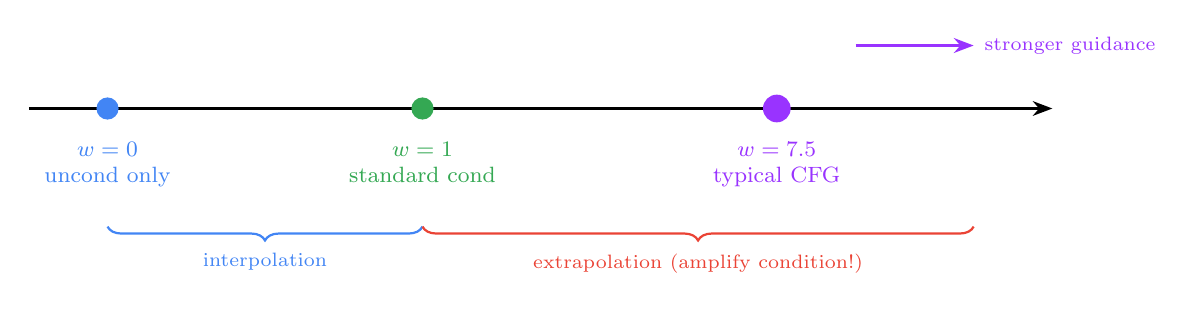
\begin{tikzpicture}[
    >={Stealth[length=2.5mm]},
    every node/.style={font=\small},
]
    % Number line
    \draw[thick, ->] (-1, 0) -- (12, 0);

    % w=0
    \fill[cblue] (0, 0) circle (4pt);
    \node[below=0.3cm, cblue, align=center, font=\footnotesize] at (0, 0) {$w=0$\\uncond only};

    % w=1
    \fill[cgreen] (4, 0) circle (4pt);
    \node[below=0.3cm, cgreen, align=center, font=\footnotesize] at (4, 0) {$w=1$\\standard cond};

    % w=7.5 typical
    \fill[cpurple] (8.5, 0) circle (5pt);
    \node[below=0.3cm, cpurple, align=center, font=\footnotesize] at (8.5, 0) {$w=7.5$\\typical CFG};

    % Regions
    \draw[decorate, decoration={brace, amplitude=5pt, mirror}, thick, cblue]
        (0, -1.5) -- (4, -1.5) node[midway, below=6pt, font=\scriptsize, cblue] {interpolation};
    \draw[decorate, decoration={brace, amplitude=5pt, mirror}, thick, cred]
        (4, -1.5) -- (11, -1.5) node[midway, below=6pt, font=\scriptsize, cred] {extrapolation (amplify condition!)};

    % Arrow showing "more aligned with condition"
    \draw[->, very thick, cpurple] (9.5, 0.8) -- (11, 0.8) node[right, font=\scriptsize] {stronger guidance};
\end{tikzpicture}
\end{center}

\bigskip

\begin{itemize}
    \item $w = 0$: Ignore the condition entirely (unconditional generation)
    \item $w = 1$: Standard conditional generation (no guidance amplification)
    \item $w > 1$: \textbf{Extrapolate} away from unconditional $\Rightarrow$ \textbf{amplify} the condition
    \item Typical values: $w \in [3, 15]$ depending on the task
\end{itemize}

\end{frame}

% ============================================================
\section{Training: How to Get Both Models in One}
% ============================================================

\begin{frame}{Training Strategy: Random Dropout of Condition}

\textbf{Key trick:} Train a \emph{single} model that can do both conditional and unconditional prediction.

\bigskip

During training, randomly replace the condition $c$ with a null token $\varnothing$ with probability $p_\text{uncond}$ (typically 10--20\%):

\begin{center}
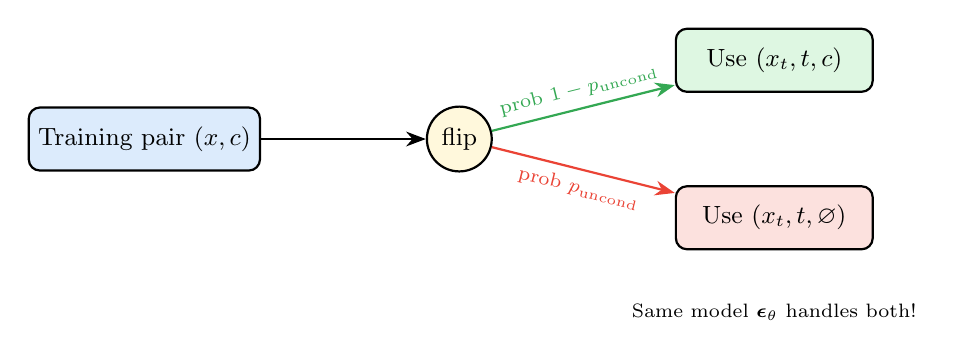
\begin{tikzpicture}[
    >={Stealth[length=2.5mm]},
    box/.style={draw, rounded corners, minimum width=2.5cm, minimum height=0.8cm, font=\small, thick},
    every node/.style={font=\small},
]
    % Training sample
    \node[box, fill=lightblue] (sample) at (0, 0) {Training pair $(x, c)$};

    % Coin flip
    \node[draw, circle, thick, fill=lightyellow, inner sep=3pt] (coin) at (4, 0) {flip};

    % Conditional path
    \node[box, fill=lightgreen] (cond) at (8, 1) {Use $(x_t, t, c)$};

    % Unconditional path
    \node[box, fill=lightred] (uncond) at (8, -1) {Use $(x_t, t, \varnothing)$};

    \draw[->, thick] (sample) -- (coin);
    \draw[->, thick, cgreen] (coin) -- node[above, font=\scriptsize, sloped] {prob $1 - p_\text{uncond}$} (cond);
    \draw[->, thick, cred] (coin) -- node[below, font=\scriptsize, sloped] {prob $p_\text{uncond}$} (uncond);

    % Brace
    \node[font=\scriptsize, align=center] at (8, -2.2) {Same model $\boldsymbol{\epsilon}_\theta$ handles both!};
\end{tikzpicture}
\end{center}

\bigskip
\textbf{Loss} (same as standard diffusion):
\[
    \mathcal{L} = \mathbb{E}_{x_0, \epsilon, t, c'}\!\left[\left\| \epsilon - \boldsymbol{\epsilon}_\theta(x_t, t, c') \right\|^2\right], \quad c' = \begin{cases} c & \text{w.p. } 1-p_\text{uncond} \\ \varnothing & \text{w.p. } p_\text{uncond} \end{cases}
\]

\end{frame}

% ============================================================
\begin{frame}{What is the Null Condition $\varnothing$?}

Different implementations handle $\varnothing$ differently:

\bigskip

\begin{center}
\renewcommand{\arraystretch}{1.6}
\begin{tabular}{lll}
\toprule
\textbf{Model} & \textbf{Condition type} & \textbf{$\varnothing$ implementation} \\
\midrule
Class-conditional & Class label $c \in \{0,\ldots,K\}$ & Extra ``null class'' ID \\
Text-to-image & Text embedding & Empty string ``\,'' embedding \\
DALL-E 2 & CLIP embedding & Zero vector \\
Stable Diffusion & Text tokens & Embedding of ``\,'' (empty) \\
\bottomrule
\end{tabular}
\end{center}

\bigskip
The key point: $\varnothing$ tells the model ``I have no condition --- just generate anything plausible.''

\end{frame}

% ============================================================
\section{Inference: How CFG Works at Generation Time}
% ============================================================

\begin{frame}{Inference: Step by Step}

At each denoising step $t = T, T-1, \ldots, 1$:

\begin{center}
\begin{tikzpicture}[
    >={Stealth[length=2.5mm]},
    box/.style={draw, rounded corners, minimum width=2.8cm, minimum height=0.8cm, font=\small, thick},
    step/.style={draw, circle, thick, fill=cpurple!20, inner sep=3pt, font=\small\bfseries},
]
    % Step 1
    \node[step] (s1) at (0, 3) {1};
    \node[box, fill=lightblue, right=0.3cm of s1] (b1) {$\boldsymbol{\epsilon}_\text{uncond} = \boldsymbol{\epsilon}_\theta(x_t, t, \varnothing)$};
    \node[font=\scriptsize, right=0.2cm of b1] {Unconditional prediction};

    % Step 2
    \node[step] (s2) at (0, 1.8) {2};
    \node[box, fill=lightgreen, right=0.3cm of s2] (b2) {$\boldsymbol{\epsilon}_\text{cond} = \boldsymbol{\epsilon}_\theta(x_t, t, c)$};
    \node[font=\scriptsize, right=0.2cm of b2] {Conditional prediction};

    % Step 3
    \node[step] (s3) at (0, 0.3) {3};
    \node[box, fill=lightyellow, right=0.3cm of s3, minimum width=7cm] (b3) {$\tilde{\boldsymbol{\epsilon}} = \boldsymbol{\epsilon}_\text{uncond} + w \cdot (\boldsymbol{\epsilon}_\text{cond} - \boldsymbol{\epsilon}_\text{uncond})$};

    % Step 4
    \node[step] (s4) at (0, -1) {4};
    \node[box, fill=lightpurple, right=0.3cm of s4, minimum width=5cm] (b4) {Use $\tilde{\boldsymbol{\epsilon}}$ to compute $x_{t-1}$ (DDPM/DDIM step)};
\end{tikzpicture}
\end{center}

\bigskip
\alert{Note:} Each step requires \textbf{two} forward passes (one unconditional, one conditional).\\
This doubles the compute cost compared to unguided sampling.

\end{frame}

% ============================================================
\begin{frame}{Visual Intuition: What CFG Does}

\begin{center}
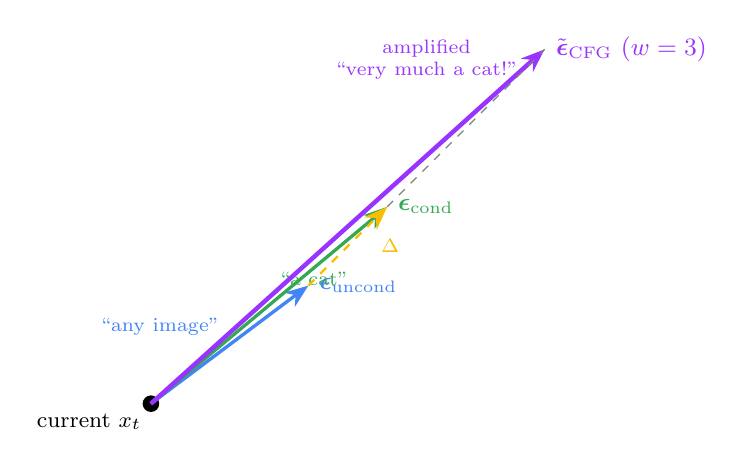
\begin{tikzpicture}[
    >={Stealth[length=3mm]},
    every node/.style={font=\small},
]
    % Origin point (current x_t)
    \fill[black] (0, 0) circle (3pt);
    \node[below left, font=\footnotesize] at (0, 0) {current $x_t$};

    % Unconditional direction
    \draw[->, very thick, cblue] (0, 0) -- (2, 1.5) node[right] {$\boldsymbol{\epsilon}_\text{uncond}$};
    \node[cblue, font=\scriptsize, above left] at (1, 0.75) {``any image''};

    % Conditional direction
    \draw[->, very thick, cgreen] (0, 0) -- (3, 2.5) node[right] {$\boldsymbol{\epsilon}_\text{cond}$};
    \node[cgreen, font=\scriptsize, below right] at (1.5, 1.8) {``a cat''};

    % Difference
    \draw[->, thick, dashed, cyellow] (2, 1.5) -- (3, 2.5);
    \node[cyellow, font=\scriptsize, right] at (2.8, 2.0) {$\Delta$};

    % CFG direction (extrapolated)
    \draw[->, ultra thick, cpurple] (0, 0) -- (5, 4.5) node[right] {$\tilde{\boldsymbol{\epsilon}}_\text{CFG}$ ($w=3$)};
    \node[cpurple, font=\scriptsize, above, align=center] at (3.5, 4) {amplified\\``very much a cat!''};

    % Dashed extension
    \draw[dashed, gray, thin] (3, 2.5) -- (5, 4.5);
\end{tikzpicture}
\end{center}

\textbf{Intuition:} CFG takes the ``direction toward condition $c$'' (the difference between conditional and unconditional predictions) and \textbf{amplifies} it by factor $w$.

\end{frame}

% ============================================================
\section{The Guidance Scale $w$: Effect and Trade-offs}
% ============================================================

\begin{frame}{Effect of Guidance Scale $w$}

\begin{center}
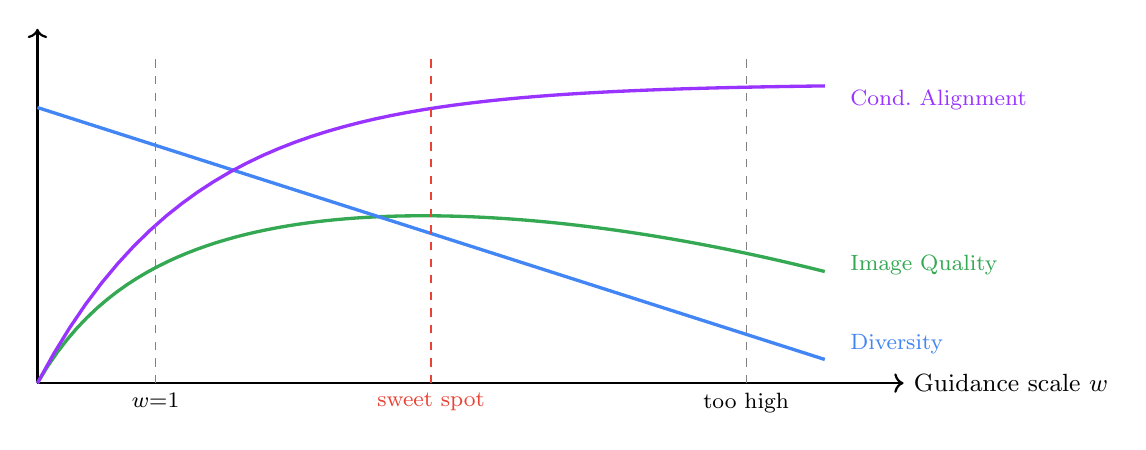
\begin{tikzpicture}[
    every node/.style={font=\small},
]
    % Axes
    \draw[->, thick] (0,0) -- (11,0) node[right] {Guidance scale $w$};
    \draw[->, thick] (0,0) -- (0,4.5);

    % Quality curve (rises then falls)
    \draw[very thick, cgreen, domain=0:10, samples=80]
        plot (\x, {3.5*\x/(2+\x) - 0.015*\x*\x});
    \node[cgreen, font=\footnotesize, right] at (10.2, 1.5) {Image Quality};

    % Diversity curve (falls)
    \draw[very thick, cblue, domain=0:10, samples=50]
        plot (\x, {3.5 - 0.32*\x});
    \node[cblue, font=\footnotesize, right] at (10.2, 0.5) {Diversity};

    % Condition alignment (rises then saturates)
    \draw[very thick, cpurple, domain=0:10, samples=50]
        plot (\x, {3.8*(1-exp(-0.5*\x))});
    \node[cpurple, font=\footnotesize, right] at (10.2, 3.6) {Cond.\ Alignment};

    % Markers
    \draw[dashed, gray] (1.5, 0) -- (1.5, 4.2);
    \node[below, font=\footnotesize] at (1.5, 0) {$w{=}1$};

    \draw[dashed, cred, thick] (5, 0) -- (5, 4.2);
    \node[below, font=\footnotesize, cred] at (5, 0) {sweet spot};

    \draw[dashed, gray] (9, 0) -- (9, 4.2);
    \node[below, font=\footnotesize] at (9, 0) {too high};
\end{tikzpicture}
\end{center}

\end{frame}

% ============================================================
\begin{frame}{Guidance Scale: Practical Examples}

\begin{center}
\renewcommand{\arraystretch}{1.6}
\begin{tabular}{cll}
\toprule
\textbf{$w$} & \textbf{Behavior} & \textbf{Analogy} \\
\midrule
$0$ & Pure unconditional generation & ``Draw whatever you want'' \\
$1$ & Standard conditional (no boost) & ``Draw a cat'' \\
$3$ & Mild guidance & ``Draw a cat, please try harder'' \\
$\mathbf{7.5}$ & \textbf{Typical for Stable Diffusion} & ``Draw a \emph{really good} cat'' \\
$15$ & Very strong guidance & ``ONLY a cat, nothing else!'' \\
$50+$ & Over-saturated, artifacts & Distorted, unnatural \\
\bottomrule
\end{tabular}
\end{center}

\bigskip
\textbf{Trade-off:}
\begin{itemize}
    \item Higher $w$ $\Rightarrow$ better alignment with condition, but less diversity and potential artifacts
    \item Lower $w$ $\Rightarrow$ more diverse, but weaker condition adherence
\end{itemize}

\end{frame}

% ============================================================
\section{Mathematical Derivation}
% ============================================================

\begin{frame}{Formal Derivation}

\textbf{Starting point:} We want to sample from $p(x_t|c)$ but amplified.

\medskip
The score of $p(x_t|c)$ using Bayes' rule:
\begin{align}
    \nabla_{x_t}\log p(x_t|c)
    &= \nabla_{x_t}\log p(x_t) + \nabla_{x_t}\log p(c|x_t) \nonumber
\end{align}

With guidance scale $s$:
\begin{align}
    \tilde{\nabla}_{x_t}
    &= \nabla_{x_t}\log p(x_t) + s \cdot \nabla_{x_t}\log p(c|x_t) \nonumber \\
    &= \nabla_{x_t}\log p(x_t) + s \cdot \big[\nabla_{x_t}\log p(x_t|c) - \nabla_{x_t}\log p(x_t)\big] \nonumber \\
    &= (1-s)\,\nabla_{x_t}\log p(x_t) + s\,\nabla_{x_t}\log p(x_t|c) \nonumber
\end{align}

Since $\boldsymbol{\epsilon}_\theta \approx -\sigma_t \nabla_{x_t}\log p(x_t)$, we translate to $\epsilon$-space (with $w = s$):

\[
\boxed{
    \tilde{\boldsymbol{\epsilon}} = \boldsymbol{\epsilon}_\theta(x_t,t,\varnothing) + w\cdot\big[\boldsymbol{\epsilon}_\theta(x_t,t,c) - \boldsymbol{\epsilon}_\theta(x_t,t,\varnothing)\big]
}
\]

This is the \textbf{Classifier-Free Guidance} formula. No classifier anywhere!

\end{frame}

% ============================================================
\begin{frame}{Connection to Implicit Classifier}

CFG \emph{implicitly} uses the diffusion model itself as a classifier:

\[
    \nabla_{x_t}\log p_\text{implicit}(c|x_t)
    \;\propto\;
    \boldsymbol{\epsilon}_\theta(x_t,t,c) - \boldsymbol{\epsilon}_\theta(x_t,t,\varnothing)
\]

\begin{center}
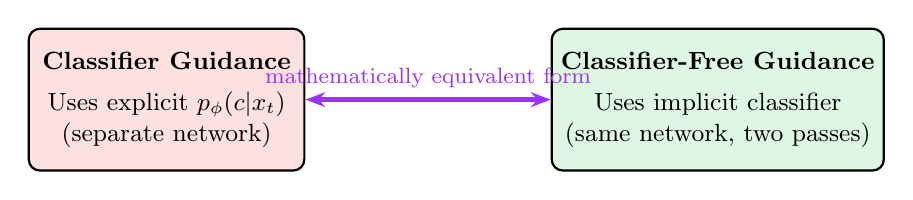
\begin{tikzpicture}[
    >={Stealth[length=2.5mm]},
    box/.style={draw, rounded corners, thick, minimum width=3.5cm, minimum height=1.8cm, align=center, font=\small},
]
    \node[box, fill=lightred] (cg) at (0, 0) {
        \textbf{Classifier Guidance}\\[4pt]
        Uses explicit $p_\phi(c|x_t)$\\
        (separate network)
    };
    \node[box, fill=lightgreen] (cfg) at (7, 0) {
        \textbf{Classifier-Free Guidance}\\[4pt]
        Uses implicit classifier\\
        (same network, two passes)
    };

    \draw[<->, ultra thick, cpurple] (cg) -- node[above, font=\footnotesize] {mathematically equivalent form} (cfg);
\end{tikzpicture}
\end{center}

\medskip
The diffusion model ``knows'' what $c$ looks like vs.\ what a generic image looks like. The \emph{difference} between the two predictions acts as an implicit classifier gradient.

\end{frame}

% ============================================================
\section{Practical Considerations}
% ============================================================

\begin{frame}{Cost: Two Forward Passes}

\alert{Main downside:} CFG requires \textbf{2 network evaluations per step}.

\begin{center}
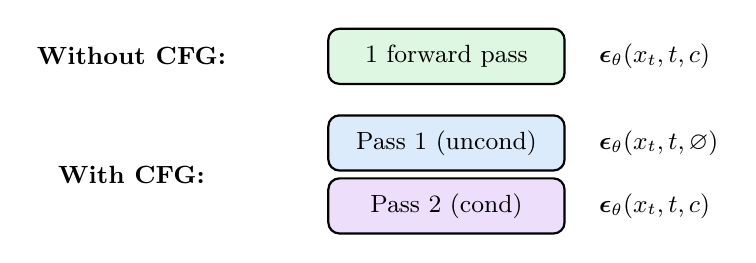
\begin{tikzpicture}[
    >={Stealth[length=2.5mm]},
    box/.style={draw, rounded corners, minimum width=3cm, minimum height=0.7cm, font=\small, thick},
]
    % Without CFG
    \node[font=\small\bfseries] at (-2, 1.5) {Without CFG:};
    \node[box, fill=lightgreen] (a1) at (2, 1.5) {1 forward pass};
    \node[font=\small, right=0.3cm of a1] {$\boldsymbol{\epsilon}_\theta(x_t, t, c)$};

    % With CFG
    \node[font=\small\bfseries] at (-2, 0) {With CFG:};
    \node[box, fill=lightblue] (b1) at (2, 0.4) {Pass 1 (uncond)};
    \node[font=\small, right=0.3cm of b1] {$\boldsymbol{\epsilon}_\theta(x_t, t, \varnothing)$};
    \node[box, fill=lightpurple] (b2) at (2, -0.4) {Pass 2 (cond)};
    \node[font=\small, right=0.3cm of b2] {$\boldsymbol{\epsilon}_\theta(x_t, t, c)$};
\end{tikzpicture}
\end{center}

\bigskip
\textbf{Optimization:} Batch both passes together --- send $[x_t, x_t]$ with conditions $[\varnothing, c]$ as a batch of size 2. This uses GPU parallelism efficiently.

\bigskip
\textbf{Distillation:} Recent work (e.g., Meng et al., 2023) trains a single model to directly predict the CFG-combined output, eliminating the double cost.

\end{frame}

% ============================================================
\begin{frame}{CFG in Popular Models}

\begin{center}
\renewcommand{\arraystretch}{1.6}
\begin{tabular}{llc}
\toprule
\textbf{Model} & \textbf{Uses CFG?} & \textbf{Typical $w$} \\
\midrule
DALL-E 2 (OpenAI) & Yes & $\sim 2$--$4$ \\
Imagen (Google) & Yes & $\sim 7$--$10$ \\
Stable Diffusion & Yes & $\sim 7.5$ (default) \\
Midjourney & Yes (variant) & Not disclosed \\
SDXL & Yes & $\sim 5$--$9$ \\
PixArt-$\alpha$ & Yes & $\sim 4.5$ \\
\bottomrule
\end{tabular}
\end{center}

\bigskip
\centering
CFG is used in \textbf{virtually all} modern text-to-image diffusion models.\\
It is one of the most impactful techniques in generative AI.

\end{frame}

% ============================================================
\section{Summary}
% ============================================================

\begin{frame}{Summary: CFG in One Slide}

\begin{center}
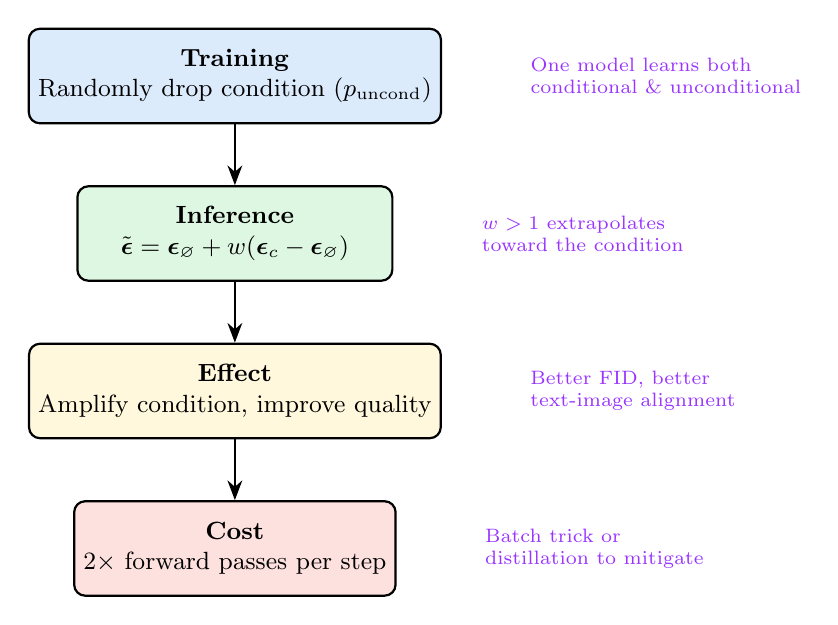
\begin{tikzpicture}[
    >={Stealth[length=2.5mm]},
    keybox/.style={draw, rounded corners, thick, minimum width=4cm, minimum height=1.2cm, align=center, font=\small},
]
    % Train
    \node[keybox, fill=lightblue] (train) at (0, 3) {
        \textbf{Training}\\
        Randomly drop condition ($p_\text{uncond}$)
    };

    % Inference
    \node[keybox, fill=lightgreen] (infer) at (0, 1) {
        \textbf{Inference}\\
        $\tilde{\boldsymbol{\epsilon}} = \boldsymbol{\epsilon}_\varnothing + w(\boldsymbol{\epsilon}_c - \boldsymbol{\epsilon}_\varnothing)$
    };

    % Effect
    \node[keybox, fill=lightyellow] (effect) at (0, -1) {
        \textbf{Effect}\\
        Amplify condition, improve quality
    };

    % Cost
    \node[keybox, fill=lightred] (cost) at (0, -3) {
        \textbf{Cost}\\
        $2\times$ forward passes per step
    };

    \draw[->, thick] (train) -- (infer);
    \draw[->, thick] (infer) -- (effect);
    \draw[->, thick] (effect) -- (cost);

    % Side annotations
    \node[font=\scriptsize, cpurple, right=1cm of train, align=left] {One model learns both\\conditional \& unconditional};
    \node[font=\scriptsize, cpurple, right=1cm of infer, align=left] {$w > 1$ extrapolates\\toward the condition};
    \node[font=\scriptsize, cpurple, right=1cm of effect, align=left] {Better FID, better\\text-image alignment};
    \node[font=\scriptsize, cpurple, right=1cm of cost, align=left] {Batch trick or\\distillation to mitigate};
\end{tikzpicture}
\end{center}

\end{frame}

% ============================================================
\begin{frame}{Key Takeaways}

\begin{enumerate}
    \item \textbf{Problem:} Conditional diffusion models need ``guidance'' to produce high-quality, condition-aligned outputs.

    \bigskip
    \item \textbf{Old solution (Classifier Guidance):} Use a separate classifier $p(c|x_t)$ to steer generation. Requires extra model, noisy-image training.

    \bigskip
    \item \textbf{CFG solution:} Train one model with random condition dropout. At inference, \textbf{extrapolate} from unconditional toward conditional prediction:
    \[
        \tilde{\boldsymbol{\epsilon}} = \boldsymbol{\epsilon}_\varnothing + w\,(\boldsymbol{\epsilon}_c - \boldsymbol{\epsilon}_\varnothing)
    \]

    \bigskip
    \item \textbf{Result:} Simple, effective, no extra models. Used in DALL-E 2, Stable Diffusion, Imagen, and almost all modern text-to-image systems.
\end{enumerate}

\end{frame}

% ============================================================
\begin{frame}{References}

\begin{itemize}
    \item \textbf{[Ho \& Salimans, 2022]} J.~Ho and T.~Salimans. ``Classifier-Free Diffusion Guidance.'' \emph{NeurIPS Workshop on DGMs}, 2022.

    \bigskip
    \item \textbf{[Dhariwal \& Nichol, 2021]} P.~Dhariwal and A.~Nichol. ``Diffusion Models Beat GANs on Image Synthesis.'' \emph{NeurIPS}, 2021.

    \bigskip
    \item \textbf{[Ho et al., 2020]} J.~Ho, A.~Jain, and P.~Abbeel. ``Denoising Diffusion Probabilistic Models.'' \emph{NeurIPS}, 2020.

    \bigskip
    \item \textbf{[Meng et al., 2023]} C.~Meng et al. ``Distillation of Guided Diffusion Models.'' \emph{CVPR}, 2023.
\end{itemize}

\end{frame}

\end{document}
